\section*{overview}
%\label{sec:prob}

We're producing a program which automatically generate metadata such as authors' name, date of publishing, name of articles... and more importantly auto-abstract for full text articles
We are interested in features for either more convenient use of the program or improving precise data generation
There are 5 related problems.\\
\begin{figure}
	\caption{The process of metadata creation}
\begin{center}
	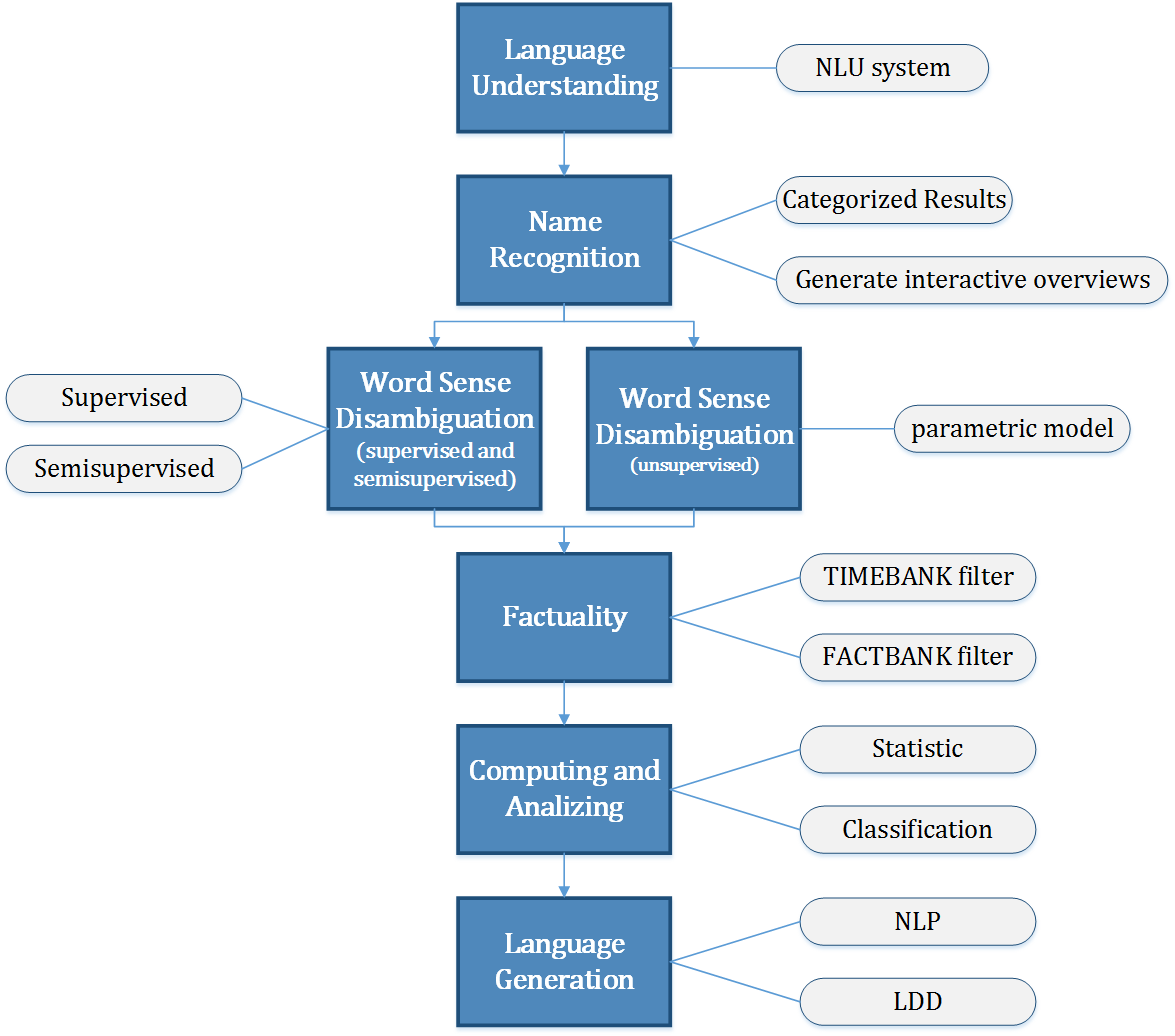
\includegraphics[width=\columnwidth]{UnionChart}
\end{center}
\end{figure}

\section*{Language understanding}

When users search with a sentence, how does the program understand the certain input of text? \\

We can build a natural language understanding (NLU) system, which uses a set of possible yes-no questions that can be applied to data items. After that, it follows a rule for selecting the best question at any node on the basis of training data by using a method for pruning trees to prevent over-training.


\section*{Name Recognition}
The results could be a country or an animal if users search for the word, Turkey.There are a lot of misunderstandings like this if users search some words which have multiply meanings. Sometimes, the results are totally unrelated and this situation is always annoying. That would be troublesome when we count frequency of a certain word to rank it. 
Therefore, it's significantly crucial for search engine to understand what users want by name recognition in natural language processing. The users can find out the results much quicker and can't get misunderstood.
The method to improve the above problem is "categorize the results based on different subjects or genres" by using online database.Metadata is limited in digital libraries and web resources, try to enlarge them with meaningful, organized and desired categories.\cite{10.1145/1141753.1141801}
Users' exploration and overviews of information could be better supported. It will be very convenient to find the results we want and lower the possibility of misunderstanding if users are not very familiar with finding the appropriate result in specific fields.\cite{DBLP:journals/jis/NaT09} Users don't have to filter the results which are ranked by browsing frequency  popularity. Users just can obtain the information and relevance by clicking the specific categories. Also, users are able to choose multiply fields if the results include a lot of relevant fields. That's a big motivation for people to handle this problems.Plus,it could be useful and interesting if people solve the problems appropriately, even perfectly.  
A lot of online services have done similar tasks before .Thus,creating and using an online database or automated metadata creation are to be recommended. The reason why is because there are some advantages, including integrating with the other cloud service or scaling with what users need such as how to categorize the categories. It is beneficial for people who would like to create a convenient and personalized database.    \\

\section*{Word sense disambiguation: supervised and semi-supervised approach}
\begin{figure}[tbh]
	\begin{center}
		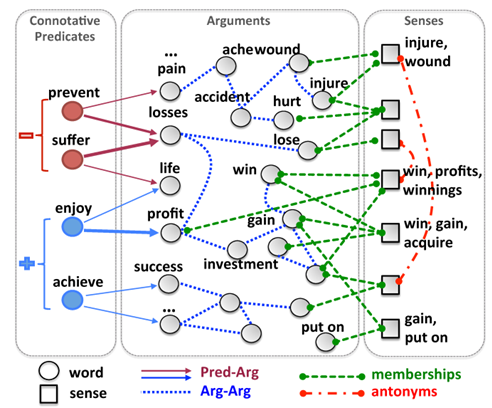
\includegraphics[width=\columnwidth]{union(WSD)}
	\end{center}
	\caption{GWord+Sense with words and senses. \label{fig1}}
\end{figure}
Word sense disambiguation (WSD) is an open problem of natural language processing and ontology. WSD is identifying which sense of a word (i.e.meaning) is used in a sentence, when the word has multiple meanings. The solution to this problem impacts other computer-related writing, such as discourse, improving relevance of search engines, anaphora resolution, coherence, inference et cetera.
The human brain is quite proficient at word-sense disambiguation. The fact that natural language is formed in a way that requires so much of it is a reflection of that neurologic reality. In other words, human language developed in a way that reflects (and also has helped to shape) the innate ability provided by the brain's neural networks. In computer science and the information technology that it enables, it has been a long-term challenge to develop the ability in computers to do natural language processing and machine learning.
\subsection*{Supervised}
\begin{figure}[tbh]
	\begin{center}
		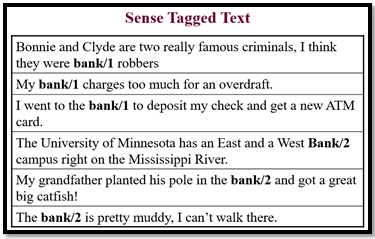
\includegraphics[width=\columnwidth]{union(sup1)}
	\end{center}
	\caption{Sense tagged text.}
\end{figure}
\begin{figure}[tbh]
	\begin{center}
		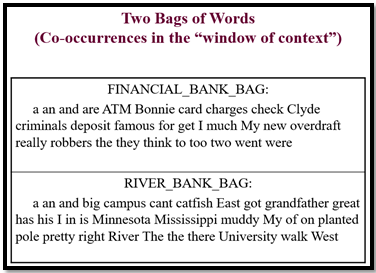
\includegraphics[width=\columnwidth]{union(sup2)}
	\end{center}
	\caption{Two bags of words.}
\end{figure}
\begin{figure}[tbh]
	\begin{center}
		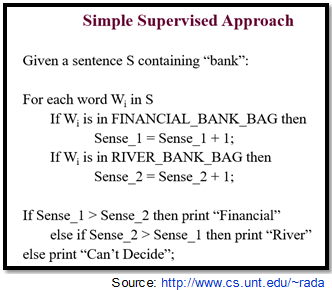
\includegraphics[width=\columnwidth]{union(sup3)}
	\end{center}
	\caption{Supervised approach.}
\end{figure}
Supervised methods are based on the assumption that the context can provide enough evidence on its own to disambiguate words (hence, common sense and reasoning are deemed unnecessary). Probably every machine learning algorithm going has been applied to WSD, including associated techniques such as feature selection, parameter optimization, and ensemble learning. Support Vector Machines and memory-based learning have been shown to be the most successful approaches, to date, probably because they can cope with the high-dimensionality of the feature space. However, these supervised methods are subject to a new knowledge acquisition bottleneck since they rely on substantial amounts of manually sense-tagged corpora for training, which are laborious and expensive to create.
\subsection*{Semi-supervised}
Because of the lack of training data, many word sense disambiguation algorithms use semi-supervised learning, which allows both labeled and unlabeled data. The Yarowsky algorithm was an early example of such an algorithm.[24] It uses the 'One sense per collocation' and the 'One sense per discourse' properties of human languages for word sense disambiguation. From observation, words tend to exhibit only one sense in most given discourse and in a given collocation.\\
\begin{figure}[tbh]
	\begin{center}
		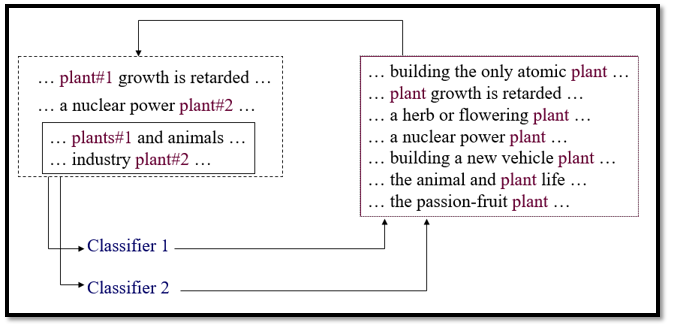
\includegraphics[width=\columnwidth]{union(semi)}
	\end{center}
	\caption{Classifier that improves over the basic classifier. \label{fig3}}
\end{figure}
The bootstrapping approach starts from a small amount of seed data for each word: either manually tagged training examples or a small number of surefire decision rules (e.g., 'play' in the context of 'bass' almost always indicates the musical instrument). The seeds are used to train an initial classifier, using any supervised method. This classifier is then used on the untagged portion of the corpus to extract a larger training set, in which only the most confident classifications are included. The process repeats, each new classifier being trained on a successively larger training corpus, until the whole corpus is consumed, or until a given maximum number of iterations is reached.\\
Other semi-supervised techniques use large quantities of untagged corpora to provide co-occurrence information that supplements the tagged corpora. These techniques have the potential to help in the adaptation of supervised models to different domains.\\
Also, an ambiguous word in one language is often translated into different words in a second language depending on the sense of the word. Word-aligned bilingual corpora have been used to infer cross-lingual sense distinctions, a kind of semi-supervised system.
\subsection*{Unsupervised}
Word Sense Disambiguation (WSD) is related to Natural Language Processing and computational languages. It came into being when people felt the need of machine translation, information retrieval, speech processing and text processing etc. The use of WSD is focused on determining the sense of word which is used in a problem by using that word in a particular context. Despite a greater number of existing disambiguation algorithms , WSD still has an open problem with the three main parts of the WSD methods being considered by literature: supervised, unsupervised and knowledge based disambiguation.
With the use of the Naive Bayes model, we can focus on the approaches to unsupervised WSD that rely on single writings. In this model, a number of sentences are used which contains a particular word which has several meanings. The main goal is to divide those words into a specified number of sense groups.
The Naive Bayes model applied mathematically entirely focuses on the issue of feature selection, which describes its two types:
\begin{enumerate}
	\item Pedersen and Bruce local type features.
	\item WordNet-based feature selection.
\end{enumerate}
Apart from the above mentioned model, the web can act as a corpus too, where it searches words which are relevant and distinctive for the target word, which makes it more appropriate in searching particular words' meaning.
So, this background focuses mainly on the issues of feature selection for unsupervised WSD performed with an underlying Naive Bayes model.


\section*{Factuality}
In the process of producing metadatas, which are should be the most precise information and representing the text, validity of such metadata must be checked. Therefore tools for fact checks are developed based on linguistic techniques.  The tool could detect facts and excludes authors' subjective opinions \cite{agerri2015big}. From this paper's perspective, the two main set of tools having such functions is TIMEBANK and FACTBANK.
TIMEBANK was first proposed in \cite{pustejovsky2003timebank}. The idea was based on that English language has different tenses which could be exploited as signals for fact check. An example as below could help clarifying the ideas. Let's examine these sentence:\\
\begin{flushleft}
	-	I will go to Chimei museum tomorrow.\\
	-	Chimei museum is near Tainan District.\\
	-	I was in UK in 2012.\\
\end{flushleft}

The first sentence is simple future tense which implying something has never actually happened, the second sentence is simple present tense which can directly imply facts, and the last sentence is in simple past tense which is about something already happened (which is facts), but is no longer a fact right now -- so such fact must be used with caution. \\

In addition to TIMEBANK, many other tools can be another filter for fact extraction. The reason for introducing such tool is that even scientific reseach articles can be glittering with subjective comments, opinions or even assumption from authors \cite{schultze2000confessional}. \cite{dave2003mining} identify words, clauses and phrases that show emotional state of the authors. The choice in expression of facts could also be a helpful indicator to show whether authors are sujectively supporting a cause, an opinion and so on \cite{wiebe2005annotating}. Among these mentioned approaches, this paper highly favors creation a kind of thesaurus compiled of linguistic signalling for non-factually statements such as FACTBANK, which is built by \cite{sauri2009factbank}. Following example shows how subjective statements can be picked out.\\
\noindent
\begin{flushleft}
	-   Channelization would guarantee high flow velocity in rivers, more flooding and consequent degradation of riparian community (1 a)\\
	-	Funding angencies would be happy with big entrepreneurs, instead of small and medium enterprises. (1 b)\\
	-	Tolerance to dictatorship would has negative influences on anarchist movement (2 a)\\
	-	Tolerance to dictatorship would doom anarchist movement. (2 c)\\
\end{flushleft}

It is easy to find in statement (1 a) is an absolute fact. Statement (1 b) is howerver affected by emotional state of authors. After re-writting (1 b) into: Funding agencies lend more money with lower interest rate to big entrepreneurs, instead of small and medium enterprises, sentence (1 b) become a face-based statement. In another case, statement (2 a) is a fact-based statement while in statement (2 b), authors are stressing their dislike toward dictatorship.\\
Fact checks in language generation is a new field but many useful tools have been developed. Each of them has their own function and could complement each others. In the limit of this study, we are using both of TIMEBANK and FACTBANK together for fact check.\\

\section*{Computing and analysing}
I suggest we should use the Python language to complete this task. 
It can easily conpute and analyze the words in the articles.
Phthon can compute and analyze by separating the connected words.
The readers can know what do the words mean when they are reading the articles .

\section*{Direction}
%\label{sec:prob}


In order to highlight the focus of the article ,the special and important words in the article need to be found mostly.
The article will promote these words to make the article's mainpoint prominent.
Compute all the words in the article and show the number of occurrences of most rankings.
By these words ,the analyzer know which words in the article should be analyzed.


\section*{Operate}
\label{sec:meth}
- distinguish     : distinguish all the words \\
\begin{center}
	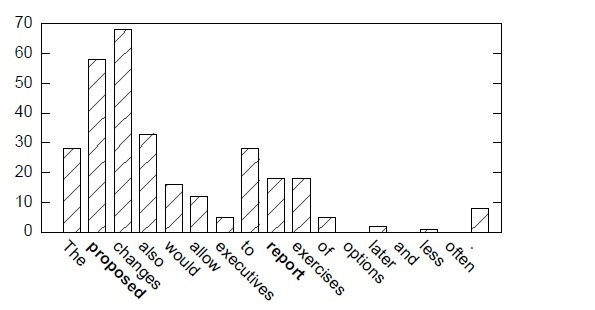
\includegraphics[width=\columnwidth]{union_01.jpg}
\end{center}
- classification   : Divided into four categories \\


a : Word Count $>$ 15 

b : 15 $>$ Word Count $>$ 10

c : 10 $>$ Word Count $>$5 

d : 5 $>$Word Count

\begin{center}
	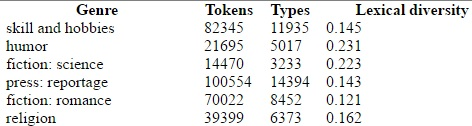
\includegraphics[width=\columnwidth]{union_02.jpg}
\end{center}
- search       \hspace{0.3cm} : Search Word repetition rate \\
- statistics   : Count the repetition rate of words \\
- sort         \hspace{0.8cm}: Show the number of rankings \\




\section*{Language generation}
%\label{sec:prob}
In the part of language generation, we would introduce two methods which are used generally in this field  \\
Natural language generation: Natural language generation is one branch of natural language processing. The goal is generating the words human being using via machine automatically. To imply this technique, six basic activities which conclude content determination, discourse planning, sentence aggregation, lexicalization, referring expression generation and linguistic realization are constructed. \cite{aramossoto2016onthe}. Some of the activities are mentioned above. The advantage of this technique is that it is flexible since there is no standardization. But it also has the difficulty in the implication of this technique.\\
Linguistic description of data: Linguistic description of data (LDD) is a concept that applied the fuzzy set theory in the linguistic field. At the beginning, the Compared to the NLG field, it is a newer technique to solve the problem of language generation. However, the basic steps of LDD have been built. The four main parts in this technique are input data, linguistic variable, fuzzy quantifiers and evaluation criteria \cite{aramossoto2016onthe}. Some of them are similar to the concept. The advantage of this technique is that it has been implied in many fields like weather forecast \cite{Ramos-SotoBBT14}. Also the many practical methods have been proposed. However, it still has a long way to go.\\
These two techniques are usually combined together nowadays. The concept of NLG and the practical approach of LDD could be used in the same time to provide the better performance in language generate field.


%
%\bibliography{Union homework
%[1].Jin 2008, Effectiveness Web Search Results for Genre and Sentiment Classification
%\\\
%[2].Bill 2006, Categorizing Web Search Results into Meaningful and Stable Categories Using Fast-Feature Techniques
%\\\
%[3].Weiscbedel 2006 White Paper on Natural Language Processing
%\\\
%[4].Collins 2011 Natural Language Processing Machine Learning Research
%\\\
%[5].Manish Gupta 2015, Information Retrieval with Verbose Queries, Foundations and Trends in Information Retrieval
%\\\
%[6].Julia Hirschberg 2015, Advances in natural language processing, Science
%\\\
%[7].Shapiro1982, A knowledge engineering approach to natural language understanding 
%\\\
%[8].Kuhn1995, The Application of Semantic Classification Trees to Natural Language Understanding
%\\\
%[9].Abualhaija, S.and Zimmermann, K.-H. 2016. D-Bees: A novel method inspired by bee colony optimization for solving word sense disambiguation. Swarm and Evolutionary Computation, 27, 188-195.
%\\\
%[10]. Ben Aouicha, M., Hadj Taieb, M. A.and Ezzeddine, M. 2016. Derivation of "is a" taxonomy from Wikipedia Category Graph. Engineering Applications of Artificial Intelligence, 50, 265-286.
%\\\
%[11]. Navigli, R. 2009. Word sense disambiguation: A survey. ACM Computing Surveys (CSUR), 41, 10. 
%\\\
%[12]. Wang, H., Missura, O., Gartner, T.and Wrobel, S. 2009. Context-based clustering of image search results. In: KI 2009: Advances in Artificial Intelligence. Springer.
%\\\
%[13]. Yoon, Y., Seon, C.-N., Lee, S.and Seo, J. 2006. Unsupervised word sense disambiguation for Korean through the acyclic weighted digraph using corpus and dictionary. Information Processing and Management, 42, 710-722.
%\\\
%Agerri, R., Artola, X., Beloki, Z., Rigau, G. and Soroa, A. 2015. Big data for Natural Language Processing: A streaming approach. Knowledge-Based Systems, 79, 36-42.
%Dave, K., Lawrence, S. and Pennock, D. M. Mining the peanut gallery: Opinion extraction and semantic classification of product reviews.  Proceedings of the 12th international conference on World Wide Web, 2003. ACM, 519-528.
%Pustejovsky, J., Hanks, P., Sauri, R., See, A., Gaizauskas, R., Setzer, A., Radev, D., Sundheim, B., Day, D. and Ferro, L. The timebank corpus.  Corpus linguistics, 2003. 40.
%Saur\'{I}, R. and Pustejovsky, J. 2009. FactBank: A corpus annotated with event factuality. Language resources and evaluation, 43, 227-268.
%Schultze, U. 2000. A confessional account of an ethnography about knowledge work. MIS Quarterly: Management Information Systems, 24, 3-40.
%Wiebe, J., Wilson, T. and Cardie, C. 2005. Annotating expressions of opinions and emotions in language. Language resources and evaluation, 39, 165-210.
